\usetikzlibrary{angles,quotes,decorations.pathreplacing}
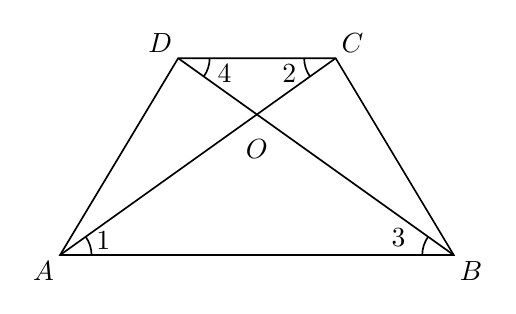
\begin{tikzpicture}[x=1cm,y=1cm,font=\normalsize,
 geometry edge/.style={solid,line width=.6pt},
 geometry mark/.style={solid,line width=.6pt},
 geometry label/.style={font=\normalsize,inner sep=2pt}]
\coordinate (A) at (0,0);
\coordinate (B) at (5,0);
\coordinate (C) at (3.5,2.5);
\coordinate (D) at (1.5,2.5);
\coordinate (O) at (2.5,1.785714);
\draw[geometry edge] (A)--(B)--(C)--(D)--cycle;
\draw[geometry edge] (A)--(C);
\draw[geometry edge] (D)--(B);
\node[font=\normalsize,inner sep=1pt] at (0.55,0.18) {$1$};
\node[font=\normalsize,inner sep=1pt] at (2.910,2.311) {$2$};
\node[font=\normalsize,inner sep=1pt] at (4.30,0.22) {$3$};
\node[font=\normalsize,inner sep=1pt] at (2.090,2.311) {$4$};
\node[geometry label,below left] at (A) {$A$};
\node[geometry label,below right] at (B) {$B$};
\node[geometry label,above right] at (C) {$C$};
\node[geometry label,above left] at (D) {$D$};
\node[geometry label,below,yshift=-7pt] at (O) {$O$};
\pic[draw,geometry mark,angle radius=4mm] {angle=B--A--C};
\pic[draw,geometry mark,angle radius=4mm] {angle=D--C--A};
\pic[draw,geometry mark,angle radius=4mm] {angle=D--B--A};
\pic[draw,geometry mark,angle radius=4mm] {angle=B--D--C};
\end{tikzpicture}
